\documentclass[conference]{IEEEtran}
\usepackage{cite}
\usepackage{amsmath,amssymb}
\usepackage{graphicx}
\usepackage{booktabs}
\usepackage[T1]{fontenc}
\usepackage[utf8]{inputenc}
\begin{document}
\title{Repeat-Sighting Diagnosis: Longitudinal Plant Health Records for a Low-Cost Agricultural Ground Robot}
\author{\IEEEauthorblockN{[Author names to be added]}\IEEEauthorblockA{[Department, Institution, City, Country] $\cdot$ [corresponding author email]}}
\maketitle
\begin{abstract}Image-based plant disease detectors usually judge one photograph at a time, so a single misclassified leaf can become a diagnosis and, on a robot, a treatment. A ground robot can do something a handheld app cannot: return to the same plant. We present C.R.A.P (Crop Robotic Autonomous Platform), a low-cost software stack that keeps a persistent health record for each plant and separates what the camera saw from what the system concludes and from what the robot does. A YOLO11s detector supplies evidence only. A transparent repeat-sighting rule marks a condition as suspected after one sighting and confirmed only after it recurs at 60\% confidence or higher, and spraying waits for human approval. An ordinary smartphone browser serves as camera and display. On 231 PlantDoc test images the detector reaches 0.663 mAP@0.5. Passing its real detections through the engine in a simulated three-visit protocol lowered wrong-condition diagnoses from 21.9\% to 17.4\% at an unchanged correct-diagnosis rate of about 50\%. With so few test images this result is suggestive and not conclusive: the 95\% bootstrap interval for the change is -9.5 to 0.0 percentage points. The benefit shrinks as errors become correlated between visits and disappears when each visit repeats the same view. We also show that a 480-pixel input matches 800-pixel accuracy at less than half the CPU latency. Trials on physical plants and on the assembled robot remain future work.\end{abstract}
\begin{IEEEkeywords}agricultural robotics, plant disease detection, object detection, YOLO, longitudinal monitoring, active perception, human-in-the-loop, precision agriculture\end{IEEEkeywords}
\section{Introduction}
Pathogens and pests take a substantial share of global food production. Savary et al. estimated mean yield losses of about 21.5\% for wheat, 30.0\% for rice, 22.5\% for maize, 17.2\% for potato and 21.4\% for soybean, based on a global survey of crop health experts \cite{savary}. Finding disease early depends on scouting, which is slow and needs trained people. This motivates automated visual inspection.

Deep learning performs very well on curated leaf images, yet this performance does not transfer easily to the field. Mohanty et al. reported 99.35\% accuracy on a held-out PlantVillage test set, but only about 31\% on images from other sources \cite{mohanty}. A 2025 review across 11 benchmark datasets reports 95--99\% laboratory accuracy against 70--85\% in field deployment \cite{shafay}. A robot acting on a single prediction inherits this gap directly: one misread leaf can trigger an unnecessary treatment.

Most systems treat each image as an independent question. A ground robot, however, can come back. We treat the return visit as the central design resource and ask whether a simple, explainable rule over a plant's history can reduce wrong diagnoses without retraining the detector.

This paper makes the following contributions:

\begin{itemize}
\item An architecture that separates evidence, judgement and action, in which every diagnosis and action is stored with its reasons in a per-plant record.
\item A transparent repeat-sighting rule, with a simple analytical model of how correlated errors limit it.
\item An evaluation that passes real detections from 231 PlantDoc test images through the implemented engine, with image-level bootstrap intervals and a correlation stress test that exposes where the rule fails.
\item A low-cost perception design using a smartphone browser and printed fiducial tags, with measurements showing that a 480-pixel input is the better operating point on a CPU.
\end{itemize}
We report both what the rule achieves and where it falls short. The evaluation is a trace-based simulation, not a field trial, and Section VII states what it cannot show.

\section{Related Work}
\subsection{Image-Based Plant Disease Recognition}
The PlantVillage repository made large-scale leaf disease learning practical \cite{hughes}, and Mohanty et al. demonstrated high accuracy on it \cite{mohanty}. Those images are largely controlled. PlantDoc added 2,598 web-sourced images across 13 species and 27 classes, with bounding boxes, to better reflect real conditions \cite{plantdoc}. Its authors reported 38.9 mAP@0.5 with Faster R-CNN Inception-ResNet v2. Ahmad et al. studied generalization across five corn disease datasets and found that models trained on laboratory images do not reach similar accuracy in the field, with a best generalization accuracy of 81.60\% \cite{ahmad}. The YOLO family reframed detection as single-pass regression \cite{redmon}, and YOLO11 refines this with C3k2 and C2PSA blocks \cite{khanam,ultralytics}.

\subsection{Field Robots for Scouting and Phenotyping}
AgriScout is a close recent example of a disease-scouting robot. It combines RGB cameras, RTK geotagging and a YOLOv11 model to find potato virus Y in commercial fields \cite{agriscout}. Young et al. built a low-cost tracked robot that measures individual energy sorghum plants \cite{young}. Atefi et al. note that robotic, non-destructive measurement allows traits of the same plant to be followed through a season \cite{atefi}. In a limited search we did not find a system that applies an explicit, per-plant confirmation rule to repeated disease detections; this is not a claim of priority, and a fuller survey is needed.

\subsection{Multiple Views and Active Perception}
Bajcsy framed perception as an active process in which a system chooses how to sense \cite{bajcsy}. Coates and Ng observed that detector errors in two images of the same scene are often different, so combining views can help, and that naively taking the strongest response can multiply false positives by the number of views \cite{coates}. They raised area under the precision-recall curve from 0.86 to 0.97 with multiple cameras and zoomed verification. They also note that correlated mistakes limit the benefit, which our stress test measures directly. Our rule uses agreement rather than the strongest response, and it does not rely on detector confidence being calibrated, a known weakness of modern networks \cite{guo}, beyond one fixed threshold.

\subsection{Targeted Treatment and Safety}
Spot spraying can reduce chemical use. In 25 hectares of sugarcane trials, robotic spot spraying used 35\% less herbicide on average while achieving about 97\% of the weed control of broadcast spraying \cite{azghadi}. These savings depend on correct targeting, so diagnosis errors matter. ISO 18497 addresses the safety of automated agricultural machinery \cite{iso}. Our approval step is a design choice in the same spirit and is not a claim of compliance.

\section{System Overview}
Fig. 1 shows the loop. A phone captures frames and displays results. A laptop runs detection and hosts the plant record, the diagnostic engine and the action manager. An ESP32 drives the robot. The modules meet only through the plant record, so each can be tested alone. This also let one software developer work in parallel with the chassis and arm teams by using a simulated robot.

\begin{figure}[t]
\centering
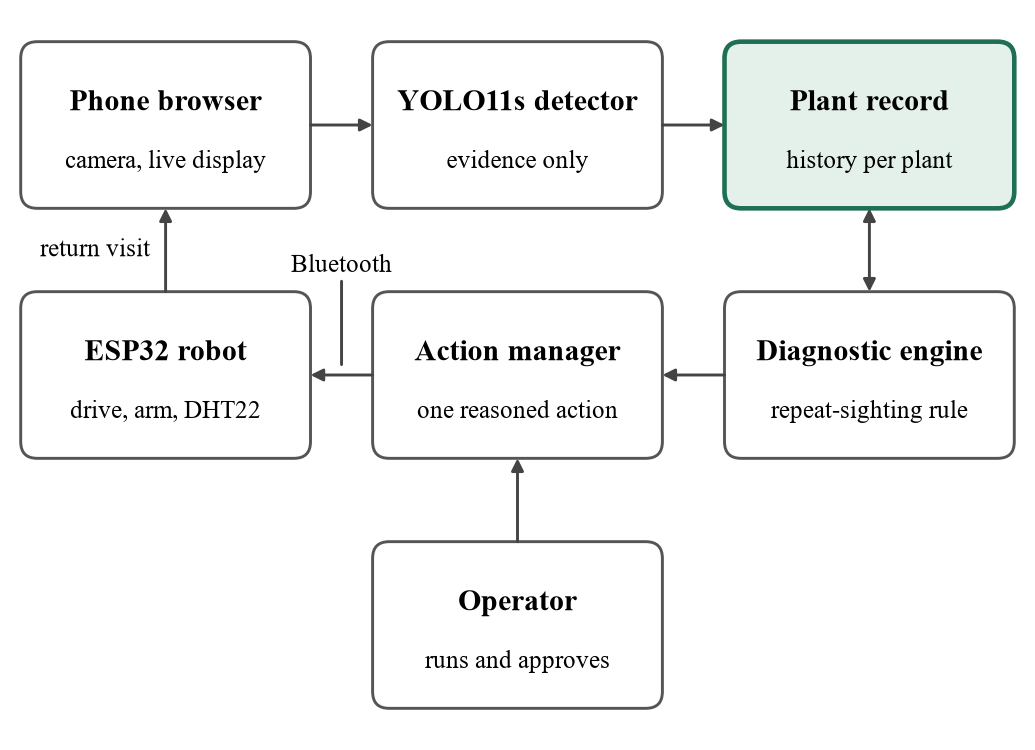
\includegraphics[width=\columnwidth]{figures/architecture.png}
\caption{System loop. Detections become evidence in the plant record. The engine judges that history, and an approved action leads to a return visit that adds new evidence.}
\end{figure}
\section{Method}
\subsection{Perception}
The detector is YOLO11s \cite{khanam,ultralytics} fine-tuned on PlantDoc for 35 epochs at 800-pixel input, with 9.42 M parameters and 21.5 GFLOPs. Its stored validation metrics are 0.602 mAP@0.5 and 0.423 mAP@0.5:0.95. The phone page sends 512-pixel-wide JPEG frames over a WebSocket and draws boxes over its own live video, so the video stays smooth even when detection is slower. Only one frame is in flight at a time, which prevents a queue from building. Mobile browsers allow camera access only on secure pages, so the laptop generates a self-signed certificate.

\subsection{Plant Identity}
A longitudinal record is useful only if the robot knows which plant it is seeing. GPS is too coarse for neighbouring plants on a low-cost robot, and visual re-identification of individual plants is difficult. We use printed ArUco markers \cite{garrido} on stakes: marker 7 maps to plant 007. The interface selects the plant when a tag is visible, with manual selection as a fallback.

\subsection{Plant Record}
Each plant stores observations, diagnoses and actions as durable JSON records. Observations retain the raw detections, so a changed rule can re-evaluate the original evidence. Each diagnosis stores supporting evidence, contradicting evidence and the observations it rests on. Live frames are not stored; only an operator-recorded visit enters the record.

\subsection{Repeat-Sighting Rule}
Let \emph{s} be the plant's species and let \emph{d}(\emph{t}, \emph{c}) be the highest confidence of condition \emph{c} among detections of species \emph{s} at visit \emph{t}, considering only detections at or above a floor of 0.35. Let $\tau$ = 0.60 be the confirmation threshold, and let \emph{H}(\emph{t}) be the last \emph{L} = 3 earlier visits with usable detections. Condition \emph{c} is confirmed at visit \emph{t} when:

\begin{equation}
d(t,c) \geq \tau \quad \text{and} \quad \exists\, u \in H(t):\ d(u,c) \geq \tau
\end{equation}
Otherwise \emph{c} remains suspected. Detections of other species are ignored and noted, because they usually reflect a misclassification or a neighbouring plant. Healthy leaves in the same image, and earlier visits that lacked \emph{c}, are recorded as contradicting evidence. Plant status is diseased if any condition is confirmed, suspected if any is suspected, healthy if only healthy leaves appear, and needs-reinspection if no usable leaves appear.

A simple model shows what the rule can and cannot do. Suppose a healthy plant produces a false sighting with probability \emph{p} per visit, and each visit repeats the previous view with probability $\rho$. The chance that two consecutive visits both produce it is:

\begin{equation}
P(\text{false confirmation}) = p\,[\,\rho + (1-\rho)\,p\,]
\end{equation}
With independent views ($\rho$ = 0) the rate falls to \emph{p}$^2$, and with identical views ($\rho$ = 1) it stays at \emph{p}. Repeating a sighting therefore helps only when the second look is genuinely different. This is why the closer inspection action below matters.

\subsection{Environmental Context}
A DHT22 sensor supplies air temperature and humidity. Disease forecasting systems for tomato and potato rely on leaf wetness and humidity \cite{rutgers}, but air humidity alone cannot diagnose disease. The engine therefore adds a note to diagnoses of humidity-favoured conditions when humidity is 70\% or higher. It never creates or confirms a diagnosis. The 70\% value is a provisional engineering choice.

\subsection{Action Lifecycle}
The action manager proposes one action per plant (Table I) and stores its reason. Nothing moves until an operator runs it, and spraying also requires explicit approval. The closer inspection links the arm to the diagnosis: it creates the second, different view that the rule needs. If any command fails, the robot is told to stop and the action is saved as failed, with the steps already completed.

\begin{table}[t]
\centering
\caption{Proposed action for each plant status}
\footnotesize
\begin{tabular}{lll}
\toprule
Status & Action & Commands \\
\midrule
Suspected & Inspect closer & Arm to inspection pose \\
Diseased & Spray (approval) & Arm to spray pose, spray 500 ms, home \\
Reinspect & Reposition, retry & Drive back 300 ms \\
Healthy & Move on & Arm home, drive forward 1 s \\
\bottomrule
\end{tabular}
\end{table}
\subsection{Robot Interface}
The robot uses one ESP32 with two L298N drivers for four DC motors, a planned four-servo arm on a PCA9685 driver, and a servo that squeezes a spray bottle trigger. The laptop sends text commands over Bluetooth Classic serial. The current firmware sends no acknowledgement and silently ignores unknown commands. Arm and spray commands are not yet in the firmware, so the software refuses those steps and reports failure rather than a false success. Every move sent has a time limit of at most 3 s.

\section{Experimental Setup}
We used the PlantDoc object detection test split \cite{plantdoc}: 231 annotated images with 447 boxes, after excluding a small number of files that could not be stored on the test machine. All timing used one Intel Core Ultra 5 125H laptop CPU with no GPU, Python 3.14 and PyTorch 2.15.

To test the rule without a field season, we used a trace-based simulation. We ran the detector once on every test image at 640-pixel input and cached the detections. A simulated plant is then a sequence of visits, each drawn from test images with that plant's true label. Healthy plants used 10 species pools and diseased plants used 17 condition pools, covering 231 single-species images. Detections passed through the implemented engine, with the plant's species known from its tag.

The baseline diagnoses a condition from a single image at the same threshold. We report three rates: correct diagnosis (the true condition is diagnosed), wrong-condition diagnosis (another condition is diagnosed on a diseased plant), and false alarm (any condition is diagnosed on a healthy plant). The engine counts a condition if it was confirmed at any visit.

Each pool holds only a few images, so simulation intervals alone would be misleadingly narrow. For the main comparison we therefore used a paired bootstrap that resamples the test images themselves (300 resamples, 200 plants per group per resample), judging the same simulated plants with both methods. Other rows use 3000 simulated plants per group. To model correlated errors, each visit repeats the previous image with probability $\rho$.

\section{Results}
\subsection{Detector Accuracy and Input Size}
Table II shows accuracy and latency by input size. Accuracy is nearly flat from 480 to 800 pixels, while latency more than doubles. At 480 pixels the model reaches 0.669 mAP@0.5 in 64 ms, against 0.659 in 148 ms at 800 pixels. The difference between these accuracies is small for a test set of this size, so we read it as equivalence and not as an advantage. For live use on a CPU, 480 pixels is the better operating point.

\begin{table}[t]
\centering
\caption{Detector accuracy and CPU latency by input size}
\footnotesize
\begin{tabular}{lllll}
\toprule
Input (px) & mAP@0.5 & mAP@.5:.95 & Mean (ms) & p95 (ms) \\
\midrule
320 & 0.644 & 0.515 & 38 & 51 \\
480 & 0.669 & 0.534 & 64 & 77 \\
640 & 0.663 & 0.530 & 97 & 114 \\
800 & 0.659 & 0.517 & 148 & 173 \\
\bottomrule
\end{tabular}
\end{table}
The result of 0.663 at 640 pixels is above the stored validation value of 0.602. The exact training split is not recorded with the weights, so some overlap with these test images cannot be ruled out, and these figures may be optimistic. It is also higher than the 38.9 originally reported on PlantDoc \cite{plantdoc}, but that used an older detector and a different class setup, so the two are not directly comparable.

Fig. 2 shows large differences between classes. Average precision ranges from 0.17 for Corn Gray leaf spot to 0.99 for Strawberry leaf. Several visually similar tomato and potato diseases score low, which matters for the wrong-condition results below.

\begin{figure}[t]
\centering
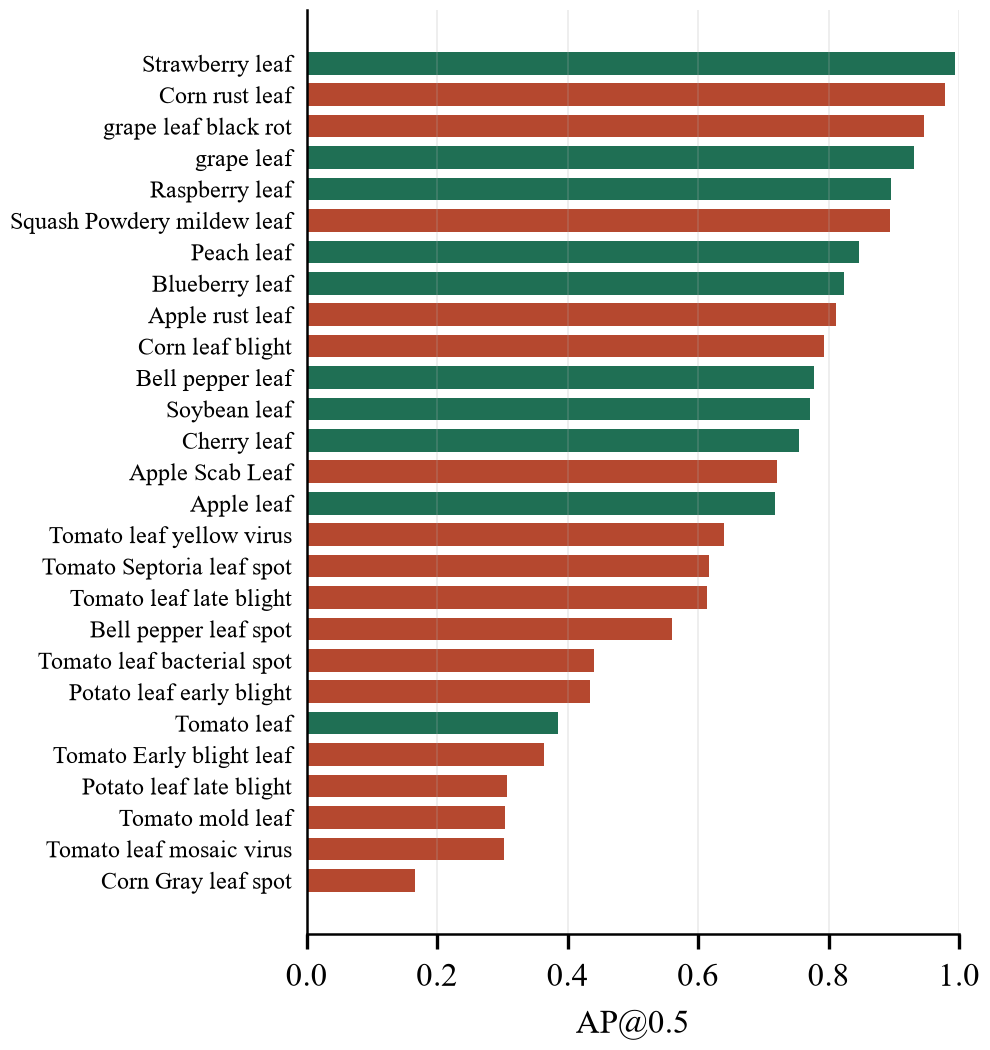
\includegraphics[width=\columnwidth]{figures/per_class.png}
\caption{Average precision by class at 800-pixel input on the test split. Green bars are healthy classes and red bars are diseases. Classes with few test images have high uncertainty.}
\end{figure}
\subsection{Pipeline Latency}
At the 640-pixel default, detection takes 97 ms, tag reading 7.4 ms and JPEG decoding 0.5 ms for a 31 KB frame. Detection therefore dominates. In an earlier end-to-end check over a local connection with the server running, the round trip averaged 166 ms, or about 6 frames per second. A browser page on the same laptop reached 3.4 to 4.7 frames per second with a simulated camera. We have not yet measured a real phone over Wi-Fi.

\subsection{Repeat Sighting Against Single-Image Diagnosis}
Table III gives the main result. With three visits, wrong-condition diagnoses fell from 21.9\% to 17.4\%, a paired change of -4.5 percentage points (95\% interval -9.5 to 0.0). Correct diagnoses changed by +0.2 points (interval -5.0 to 5.5). False alarms changed from 1.2\% to 0.7\%, a change of -0.5 points (interval -2.5 to 1.0).

These intervals call for caution. The reduction in wrong-condition diagnoses appeared in 96\% of resamples, but its interval reaches zero, so we treat it as suggestive and not as established. The correct-diagnosis rate did not measurably change, and false alarms are too rare here to separate the two methods.

\begin{table}[t]
\centering
\caption{Three-visit repeat sighting against one image at a 0.60 threshold (paired image bootstrap, mean and 95\% interval, \%)}
\footnotesize
\begin{tabular}{lll}
\toprule
Rate & Single image & Repeat sighting \\
\midrule
Correct & 50.1 (40.5 to 61.0) & 50.3 (39.0 to 61.0) \\
Wrong condition & 21.9 (13.5 to 30.5) & 17.4 (9.5 to 26.5) \\
False alarm & 1.2 (0.0 to 4.5) & 0.7 (0.0 to 4.5) \\
\bottomrule
\end{tabular}
\end{table}
The number of visits sets a trade-off. Because the engine counts a confirmation at any visit, more visits give more chances to be right and to be wrong. With 3000 simulated plants per group, two visits gave 34.2\% correct and 8.4\% wrong; three gave 48.6\% and 16.0\%; four gave 61.0\% and 21.7\%. A confirmed wrong condition therefore does not disappear with more looking. When a detector systematically confuses two diseases, the same wrong label can recur.

Raising the single-image threshold is the obvious alternative, and Fig. 3 compares both methods as the threshold varies. A single image at $\tau$ = 0.70 gave 44.2\% correct and 16.3\% wrong. Across most of the range the repeat-sighting curve lies to the left, with fewer wrong diagnoses at a similar correct rate. The two curves come close at the extremes.

\begin{figure}[t]
\centering
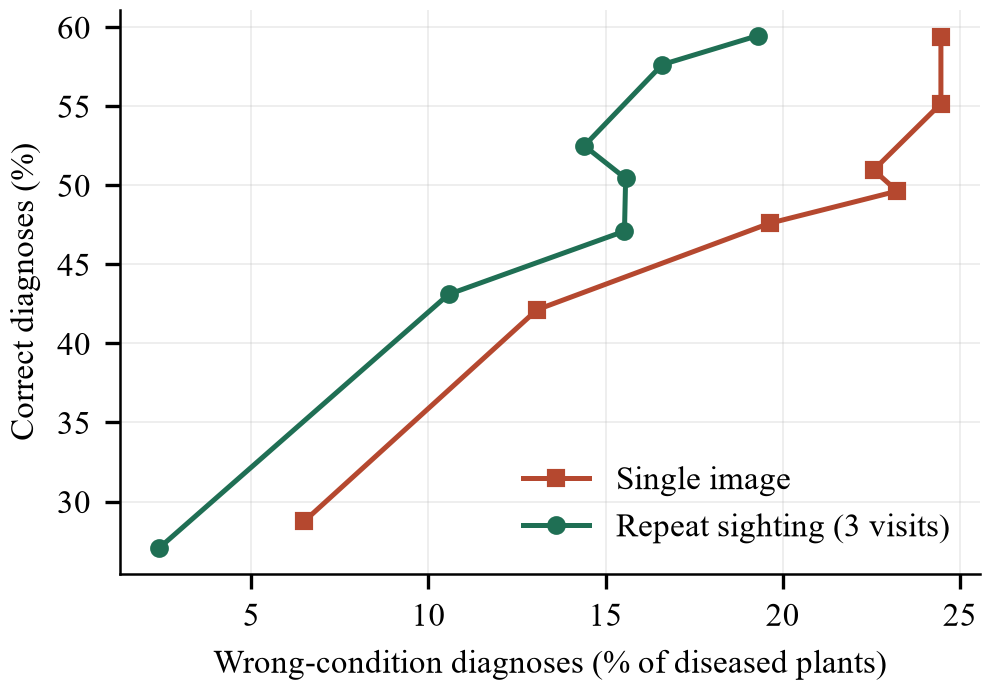
\includegraphics[width=\columnwidth]{figures/tradeoff.png}
\caption{Correct against wrong-condition diagnoses as the threshold varies from 0.35 to 0.85. Up and to the left is better.}
\end{figure}
\subsection{Correlated Errors}
Fig. 4 shows the stress test. As $\rho$ rises from 0 to 1, wrong-condition diagnoses rise from 16.1\% to 22.2\%, and false alarms rise from 0.4\% to 1.4\%. At $\rho$ = 1 the rule performs no better than a single image, as Eq. 2 predicts. Repeat sighting is therefore only as good as the independence of its views. Note that drawing from small pools already repeats some images at $\rho$ = 0, so even the best case here is not fully independent.

\begin{figure}[t]
\centering
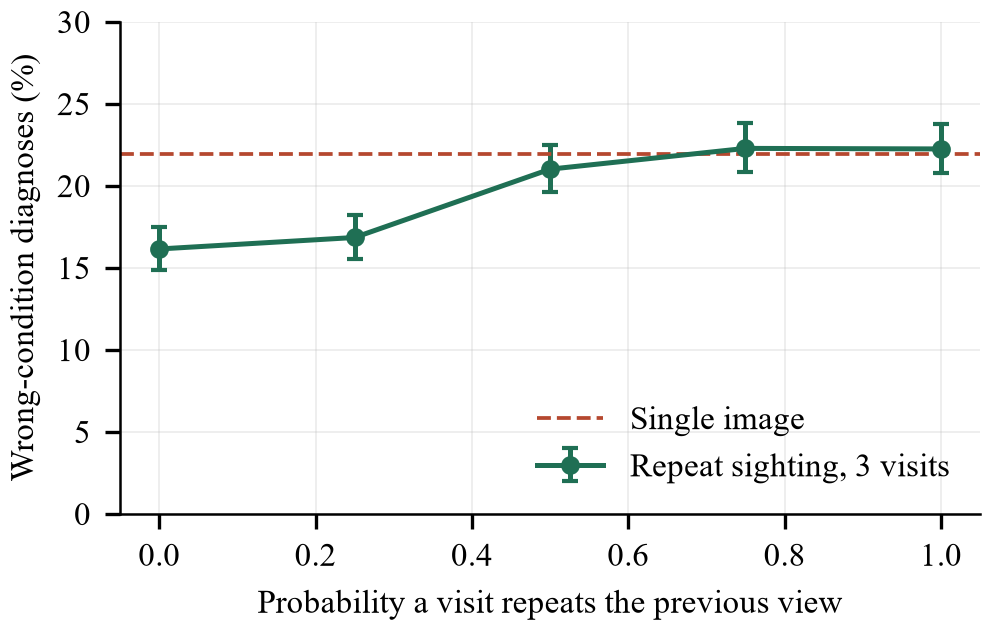
\includegraphics[width=\columnwidth]{figures/correlation.png}
\caption{Wrong-condition diagnoses as views become correlated (three visits, $\tau$ = 0.60). Error bars are 95\% Wilson intervals over simulated plants.}
\end{figure}
\subsection{Plant Tags and Software Verification}
In a synthetic test, tags pasted onto leaf images with noise and optional blur were read in 543 of 560 trials, with at least 92\% in every setting from 16 to 128 pixels. Misses did not depend clearly on size, and we did not investigate their cause. This test has no perspective, shadow or dirt, so it is an upper bound on field performance.

An automated suite of 83 tests passes. It covers persistence across restarts, the suspected-to-confirmed path, approval blocking, failure handling, the humidity rule and the Bluetooth command format. The Bluetooth link was tested against a simulated port.

\section{Discussion and Limitations}
The main finding is modest. A rule that needs no retraining and can be read in one line appears to reduce wrong diagnoses at the same correct rate, but the evidence is not yet conclusive, and most wrong diagnoses remain. Repeat sighting filters random errors, and it cannot correct a systematic confusion. With roughly half of diseased plants correctly diagnosed in this setting, the detector remains the larger constraint.

Several limitations bound these conclusions:

\begin{itemize}
\item No field trial. Simulated visits draw different web images, not repeated views of one plant. Real revisits may be more correlated, or may show disease progressing.
\item Small pools. Some conditions have as few as 3 test images.
\item Possible test overlap, since the training split is not recorded with the weights.
\item No expert ground truth. Labels come from the dataset, not from laboratory confirmation.
\item Domain gap. PlantDoc images come from the web and may not match this robot's camera.
\item Hardware. The robot was not assembled and tested for this study, and arm and spray commands are not yet in the firmware. No phone-over-Wi-Fi measurement exists.
\item Untuned thresholds. The 0.35, 0.60, three-visit and 70\% humidity values are initial choices.
\item Dependence on a laptop and a shared network, which limits field use.
\end{itemize}
\section{Conclusion and Future Work}
We presented a low-cost plant health system that treats diagnosis as record keeping over repeated visits, not as a one-photo decision. Using real detections, a simple repeat-sighting rule showed a suggestive reduction in wrong-condition diagnoses at an unchanged correct rate, and a correlation test showed when that benefit disappears. Compared with 800 pixels, a 480-pixel input more than halved CPU latency with no measurable loss of accuracy.

The next step is a controlled trial on real plants with expert labels, comparing same-view revisits with arm-driven closer views to measure real error correlation. Further work includes firmware support for the arm, a tagged-row route for autonomous visits, per-class thresholds, on-phone inference, and using low-confidence frames to retrain the model on local fields.

\section*{Acknowledgment}
The authors thank the C.R.A.P chassis, arm and perception team members. [Add funding and supervisor acknowledgements.]
\begin{thebibliography}{99}
\bibitem{savary} S. Savary, L. Willocquet, S. J. Pethybridge, P. Esker, N. McRoberts, and A. Nelson, ``The global burden of pathogens and pests on major food crops,'' \emph{Nature Ecology \& Evolution}, vol. 3, pp. 430--439, 2019.
\bibitem{mohanty} S. P. Mohanty, D. P. Hughes, and M. Salathé, ``Using deep learning for image-based plant disease detection,'' \emph{Frontiers in Plant Science}, vol. 7, art. 1419, 2016.
\bibitem{shafay} M. Shafay, T. Hassan, M. Owais, I. Hussain, S. G. Khawaja, L. Seneviratne, and N. Werghi, ``Recent advances in plant disease detection: challenges and opportunities,'' \emph{Plant Methods}, vol. 21, no. 1, art. 140, 2025.
\bibitem{hughes} D. P. Hughes and M. Salathé, ``An open access repository of images on plant health to enable the development of mobile disease diagnostics,'' arXiv:1511.08060, 2015.
\bibitem{plantdoc} D. Singh, N. Jain, P. Jain, P. Kayal, S. Kumawat, and N. Batra, ``PlantDoc: A dataset for visual plant disease detection,'' in \emph{Proc. ACM CoDS-COMAD}, 2020, pp. 249--253.
\bibitem{ahmad} A. Ahmad, A. El Gamal, and D. Saraswat, ``Toward generalization of deep learning-based plant disease identification under controlled and field conditions,'' \emph{IEEE Access}, vol. 11, pp. 9042--9057, 2023.
\bibitem{redmon} J. Redmon, S. Divvala, R. Girshick, and A. Farhadi, ``You only look once: Unified, real-time object detection,'' in \emph{Proc. IEEE CVPR}, 2016, pp. 779--788.
\bibitem{khanam} R. Khanam and M. Hussain, ``YOLOv11: An overview of the key architectural enhancements,'' arXiv:2410.17725, 2024.
\bibitem{ultralytics} G. Jocher and J. Qiu, \emph{Ultralytics YOLO11}, software, Ultralytics, 2024. [Online]. Available: https://github.com/ultralytics/ultralytics
\bibitem{agriscout} C. Singh \emph{et al.}, ``AgriScout: AI-powered robot for precise detection of PVY-infected potato plants,'' \emph{Computers and Electronics in Agriculture}, vol. 238, art. 110781, 2025.
\bibitem{young} S. N. Young, E. Kayacan, and J. M. Peschel, ``Design and field evaluation of a ground robot for high-throughput phenotyping of energy sorghum,'' \emph{Precision Agriculture}, vol. 20, no. 4, pp. 697--722, 2019.
\bibitem{atefi} A. Atefi, Y. Ge, S. Pitla, and J. Schnable, ``Robotic technologies for high-throughput plant phenotyping: Contemporary reviews and future perspectives,'' \emph{Frontiers in Plant Science}, vol. 12, art. 611940, 2021.
\bibitem{bajcsy} R. Bajcsy, ``Active perception,'' \emph{Proceedings of the IEEE}, vol. 76, no. 8, pp. 966--1005, 1988.
\bibitem{coates} A. Coates and A. Y. Ng, ``Multi-camera object detection for robotics,'' in \emph{Proc. IEEE ICRA}, 2010.
\bibitem{guo} C. Guo, G. Pleiss, Y. Sun, and K. Q. Weinberger, ``On calibration of modern neural networks,'' in \emph{Proc. ICML}, 2017, pp. 1321--1330.
\bibitem{azghadi} M. Rahimi Azghadi \emph{et al.}, ``Precision robotic spot-spraying: Reducing herbicide use and enhancing environmental outcomes in sugarcane,'' \emph{Computers and Electronics in Agriculture}, vol. 235, art. 110365, 2025.
\bibitem{iso} ISO 18497, \emph{Agricultural machinery and tractors: Safety of partially automated, semi-autonomous and autonomous machinery}, International Organization for Standardization, 2024.
\bibitem{garrido} S. Garrido-Jurado, R. Muñoz-Salinas, F. J. Madrid-Cuevas, and M. J. Marín-Jiménez, ``Automatic generation and detection of highly reliable fiducial markers under occlusion,'' \emph{Pattern Recognition}, vol. 47, no. 6, pp. 2280--2292, 2014.
\bibitem{rutgers} Rutgers Cooperative Extension, ``Potato and tomato disease forecasting,'' \emph{Plant \& Pest Advisory}. [Online]. Available: https://plant-pest-advisory.rutgers.edu
\end{thebibliography}
\end{document}